\documentclass{article}
\usepackage[minionint,mathlf,textlf]{MinionPro} % To gussy up a bit
\usepackage[margin=1in]{geometry}
\usepackage{graphicx} % For .eps inclusion
%\usepackage{indentfirst} % Controls indentation
\usepackage[compact]{titlesec} % For regulating spacing before section titles
\usepackage{adjustbox} % For vertically-aligned side-by-side minipages
\usepackage{array, mathrsfs, mathrsfs, mhchem, amsmath} % For centering of tabulars with text-wrapping columns
\usepackage{hyperref, chemfig}
\usepackage{subfigure}
\usepackage[autolinebreaks,framed,numbered]{mcode}
\newcommand{\Lapl}{\mathscr{L}}

\pagenumbering{gobble} 
\setlength\parindent{0 cm}
\begin{document}
\large

\section*{Evolvability: opsin and olfactory receptor selection}

The architecture of a system can determine how easily it can be expanded through the course of evolution. Consider, for example, the developmental system which generates photoreceptors of different subtypes. The human retina has one type of rod and three types of cones: each type expresses a unique opsin gene and therefore has a different absorption spectrum. The cones, which are involved in color vision, are often labeled blue (short wavelength or SW), green (MW), and red (LW). During development, the opsin which a photoreceptor will express is chosen with some degree of randomness, so that any reasonably large and central field of vision should have a mix of red, green, and blue cones for color detection as well as rods for edge and motion detection. While the ratio is not constant between persons or even within a single retina, a mechanism clearly exists for expressing one opsin gene at the expense of all others.
\begin{center}
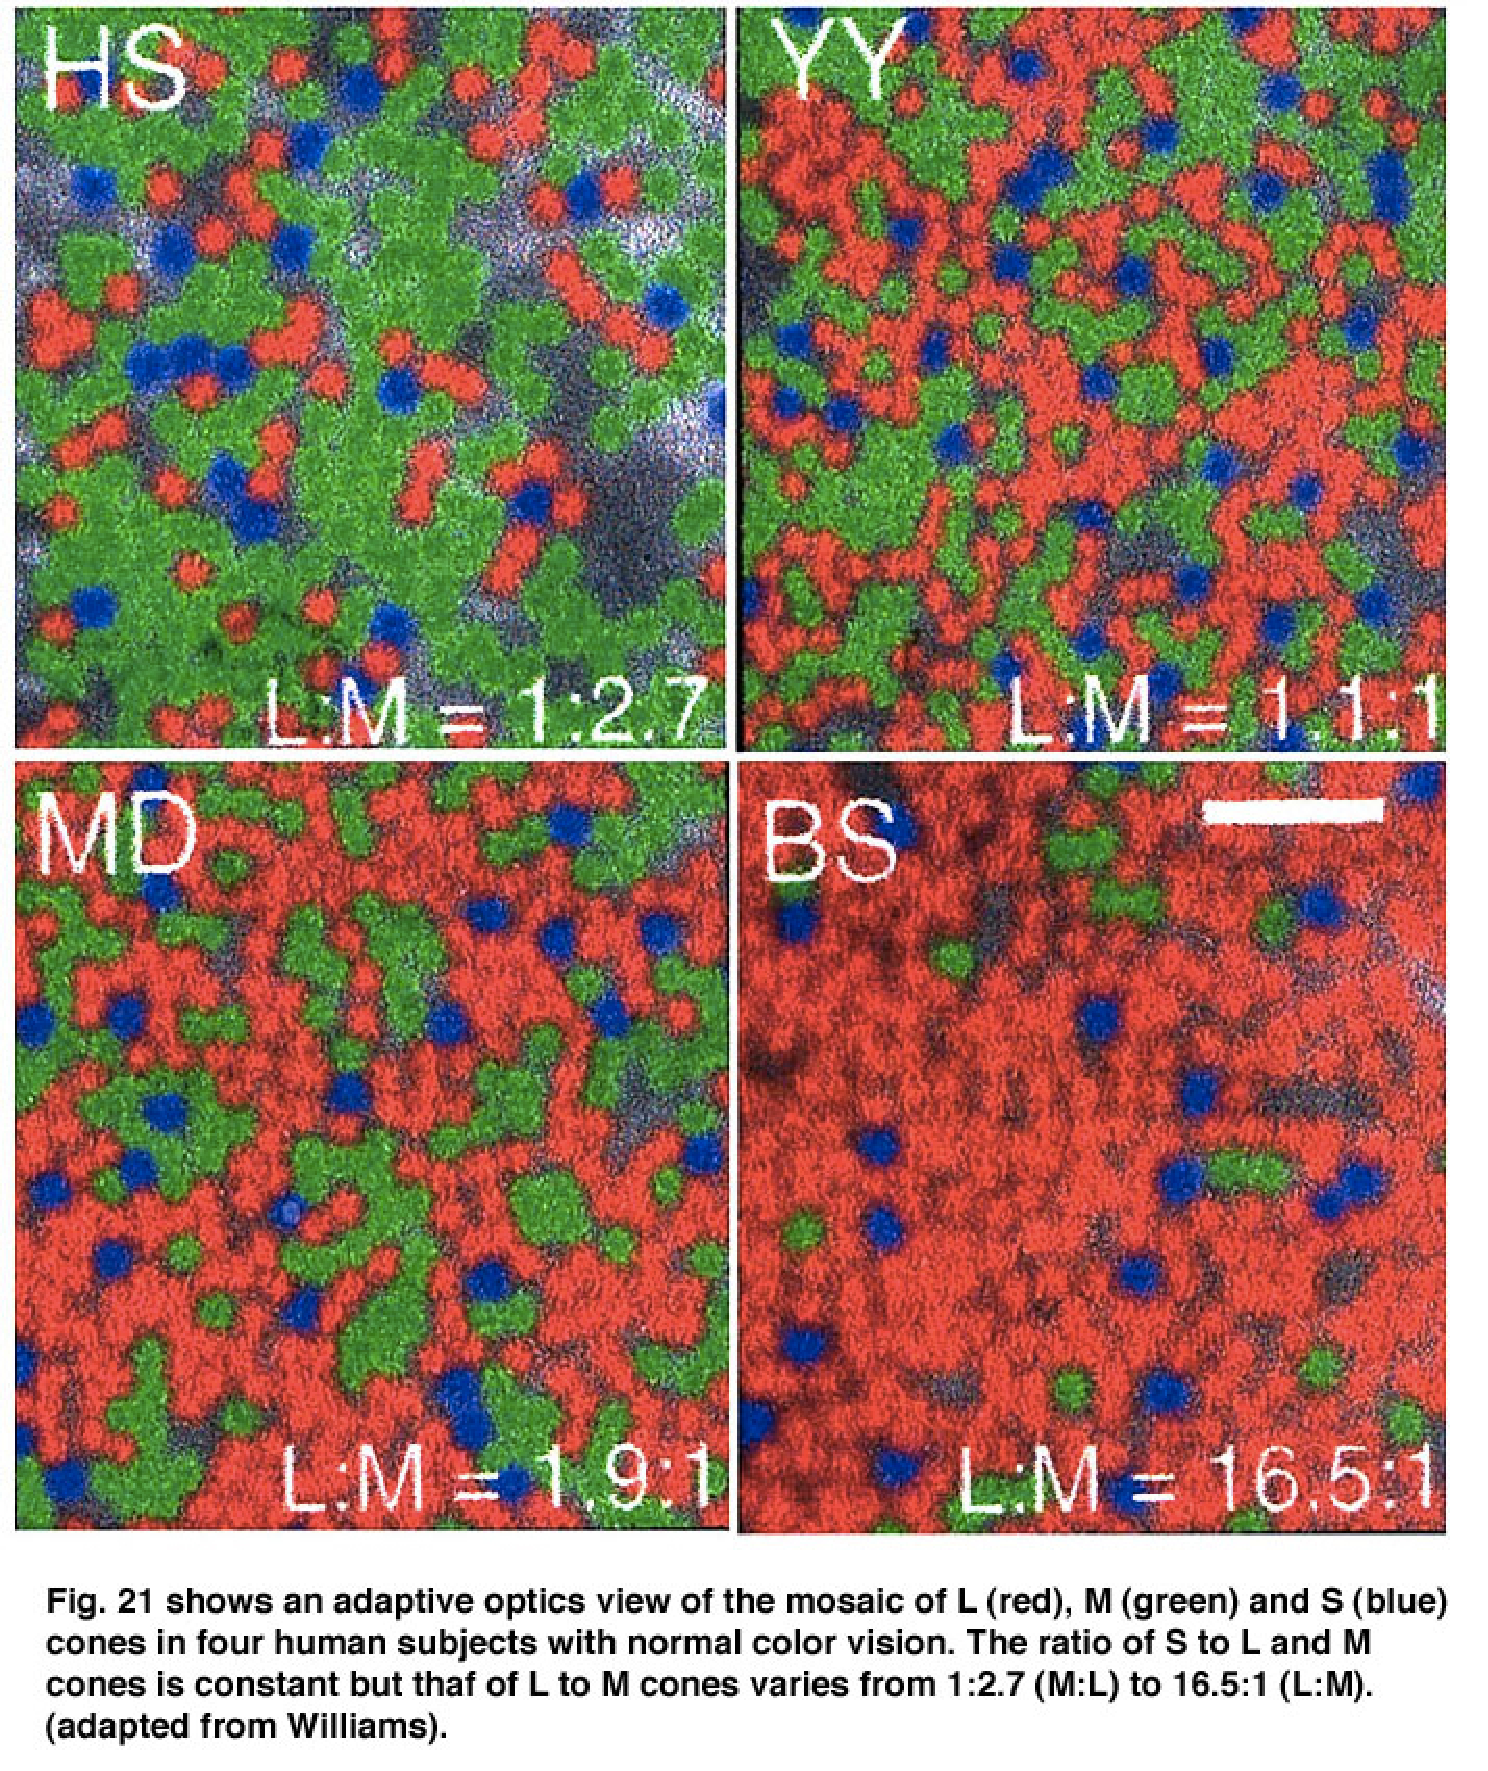
\includegraphics[width=0.4\textwidth]{distribution.pdf}
\end{center}
Given what you have learned about switches and spatial patterning so far in the course, you may already have some ideas for how to generate a mix of cell types from an initially equivalent field of photoreceptor precursors. Developmental studies suggest that all photoreceptor precursors express the blue opsin at first: a subset of these cells then differentiate to express rhodopsin instead and become rods. Another subset diverges from the blue opsin-expressing cones to become red-green cones. Both of these genes are located on the X chromosome: due to X inactivation, the decision of whether to express the red vs. green opsin is apparently made through association of a promoter region on the active X with either a red or green opsin in \textit{cis}.\\

Most non-primate mammals have only rhodopsin and blue and green opsin genes\footnote{The story goes that red opsin evolved in our lineage due to selective pressure on frugivores to identify ripe fruit. Angiosperms, the flowering and fruit-producing plants, rose to dominance only about 100 million years ago; the primates diverged about 65 million years ago.}. Even with this bare-bones understanding of photoreceptor development, it is clear that inserting a fourth opsin into the patterning system via would have been a much more involved affair if it were not for the fortuitous circumstances of green opsin. The location of the locus control region (LCR) on the X chromosome ensures that only one activator is driving a red/green opsin; anywhere else in the genome, there may have been two LCRs each operating on homologous chromosomes, potentially choosing different opsins\footnote{Although this would be a problem in the ``one photoreceptor, one opsin" pattern, some mammals including mice express multiple color opsins in the same cone.}. It is also very fortunate that the LCR should form a permanent association with either the red or green opsin promoter, since if it were to switch between them, a cone would express a mixture of red and green opsins.

\begin{center}
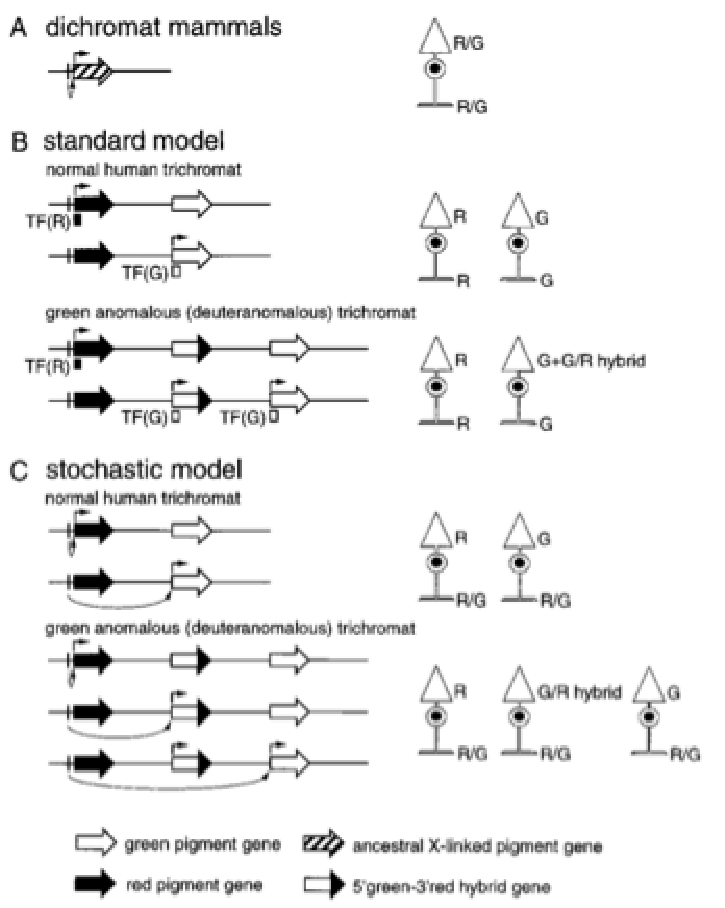
\includegraphics[width=0.4\textwidth]{lcr_stochastic.pdf}
\end{center}


The relatively self-contained nature of the red vs. green opsin choice is made clear through experimentation. When a single copy of the human LCR and different reporters in place of the red- and green- opsins are cloned into mice, most cones express only one report, not both (Wang et al., 1999). Other organisms such as zebrafish in which opsin duplications have occurred also limit expession to a single allele in part via a shared enhancer (Tsujimura et al., 2010)\footnote{This case is a bit more complicated, since the opsin paralogs and locus control regiona are not on a sex chromosome. One opsin or the other is favored by spatial context.}.

\begin{center}
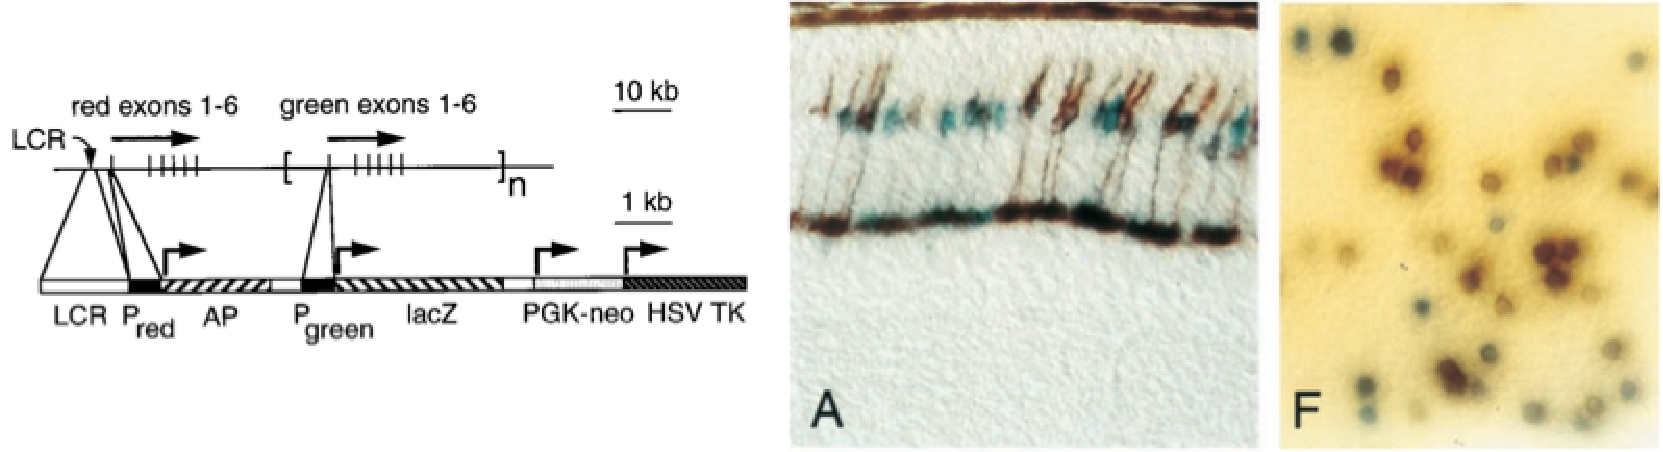
\includegraphics[width=0.8\textwidth]{lcr_in_mice.pdf}
\end{center}

Why is it that in some people the ratios between red and green cones can be so highly variable (Roorda and Williams, 1999), even among males? The duplication event that created the green and red opsins in tandem also permits unequal recombination between sister chromatids that can add or remove copies of these alleles. These errors are at the root of red-green color blindness (deuteranopia and protoanopia) which result from functional loss of one opsin. Similar crossover errors can partially convert e.g. a red gene to a green one and give rise to the more subtle variations in red and green color vision referred to as proto- and deuteranomaly. The causes of variation in red-to-green cone ratios may be more subtle, but as far as I'm aware the histological ratio between red and green cones has never been compared to the number of copies of each gene type\footnote{Patient-reported color discrimination suggests that these extra gene copies farther from the LCR are not expressed highly enough to influence perception, but it is possible that copy number is partially compensated by visual processing.}.

\begin{center}
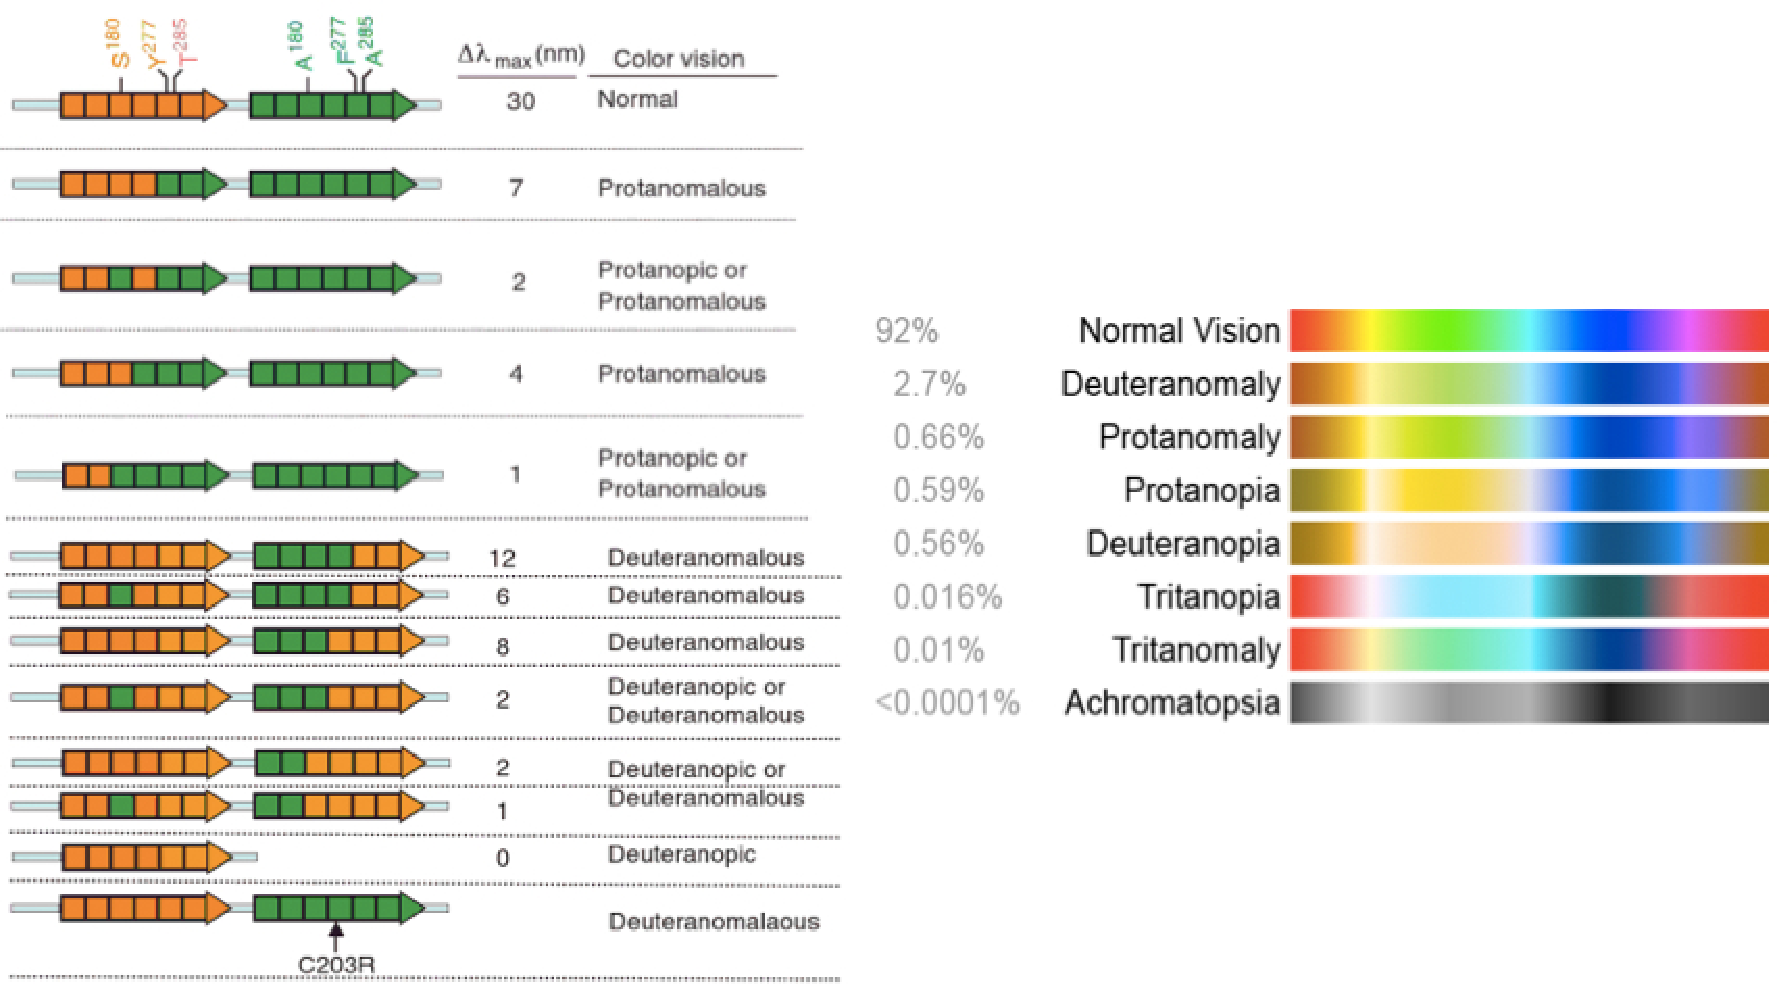
\includegraphics[width=0.8\textwidth]{anomalies.pdf}
\end{center}

New World primates have evolved red and green opsins through a separate event: mutation of an X-linked opsin to produce a second allele with different absorbance spectrum. Both alleles have been maintained in the population, though only females heterozygous for the red and green opsins have the benefit of trichromatic vision.

\begin{center}
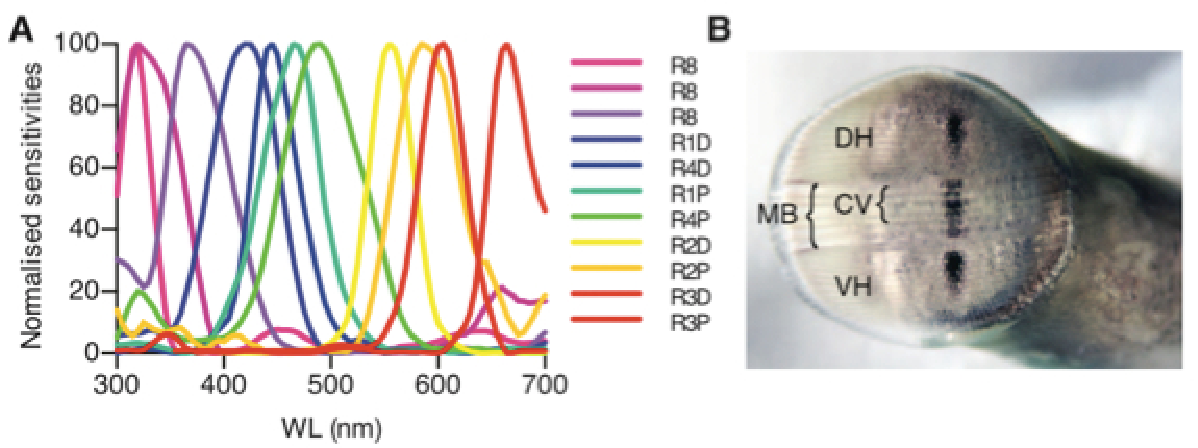
\includegraphics[width=0.4\textwidth]{mantis_opsins.pdf}
\end{center}

Some crustaceans and insects have dozens of opsin genes. In the case of mantis shrimp, twelve types of color photoreceptors are laid out in rows with characteristic sensitivities. The advantage of this arrangement appears to be that rather than performing comparisons between the output of each type of photoreceptor, with a quick eye movement the shrimp can ``scan" the image over the array of photoreceptors, creating a temporal signature indicative of the object's color (Thoen et al., 2014). Whether this developmental system is extensible remains unclear, though the large number of photoreceptor types involved favors a labile mechanism over a hard-wired one.

\begin{center}
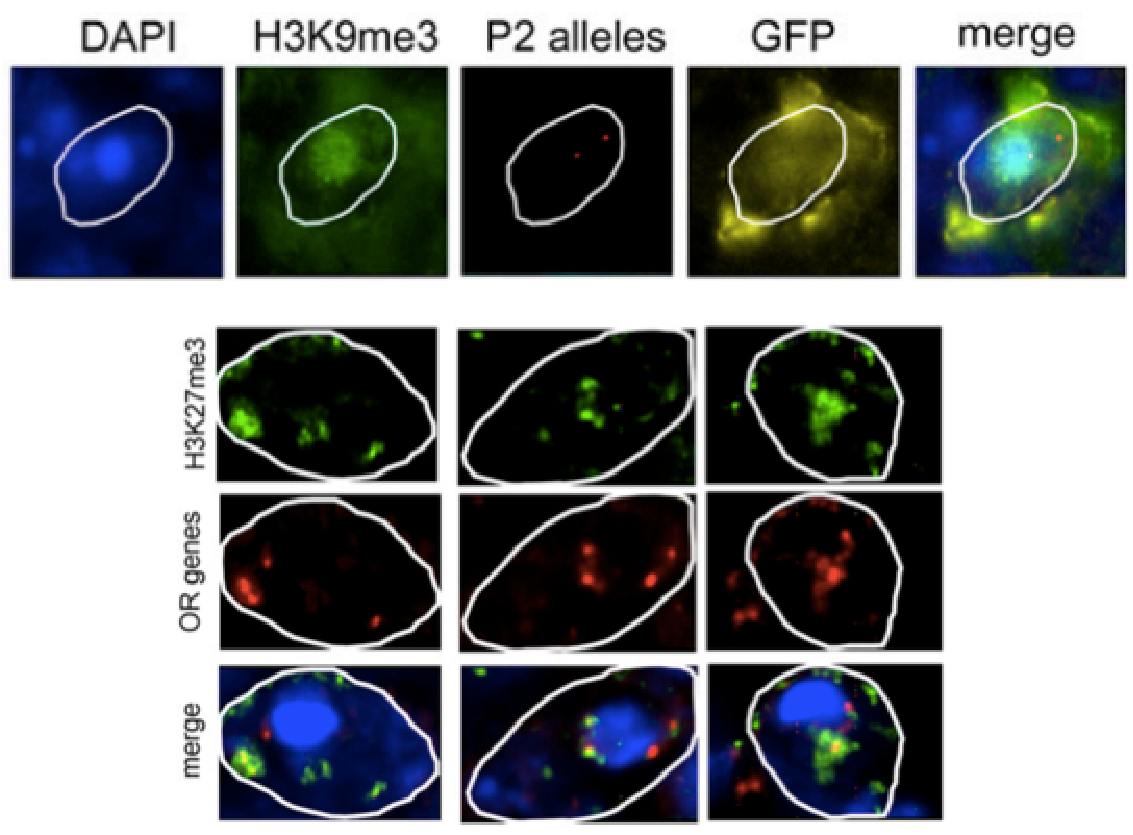
\includegraphics[width=0.6\textwidth]{or_localization.pdf}
\end{center}

By contrast to opsins, humans have about nine hundred genes encoding olfactory receptors spread throughout the genome. As in the visual system, each olfactory sensory neuron appears to express precisely one of these 1800 alleles. Clearly an extensible system is in place here to ensure that only one of many genes is expressed. Although the receptor selection mechanism is not fully understood, some details provide a rough sketch. Despite substantial divergence, the promoter regions of olfactory receptors are remarkably conserved for non-coding regions, with shared regulatory elements (Clowney 2011). The interaction of multiple enhancer elements spread across some six chromosomes may be necessary to drive transcription of an OR gene (Markenscoff-Papadimitriou 2014).
The receptor choice appears to be ``locked in" through epigenetic modifications that relegate the other olfactory receptor alleles to heterochromatin and particular regions of the nucleus (Clowney 2012).

\section*{Modularity and load management}

A module is a self-contained set of elements that carries out some function and can be linked to others through a clearly-defined set of inputs or outputs. For example, a Delta-Notch signaling system can be pictured as a functional module with an ``output" given by the concentration of the transcriptional regulator NICD. We can ``hook up" other functions to this output as you saw in the reporter labeling of Notch+ and Delta+ cells in Matsuda et al. 2015 (lecture 26). Typically we call something a module only if the input/output interactions can be readily recreated synthetically, such as gene regulation through a known operator or addition of a self-folding regulatory domain to a protein.\\

New functionality can be evolved through the establishment of new connections between existing modules without requiring duplication and divergence. However, just as connecting many strings of Christmas lights to the same outlet can overload a circuit, connecting too many downstream modules to the same input can impair its functionality. For example, if the output of the upstream circuit is a transcription factor, including more binding sites than transcription factor proteins would limit the probability of binding at any one site. Even when the number of binding sites is not larger than the protein count, as we will see below, those extra binding sites can ``buffer" the free protein concentration against changes in protein production rate. This effect of newly-added downstream components on the functioning of the existing system is called \textit{retroactivity}.

\begin{center}
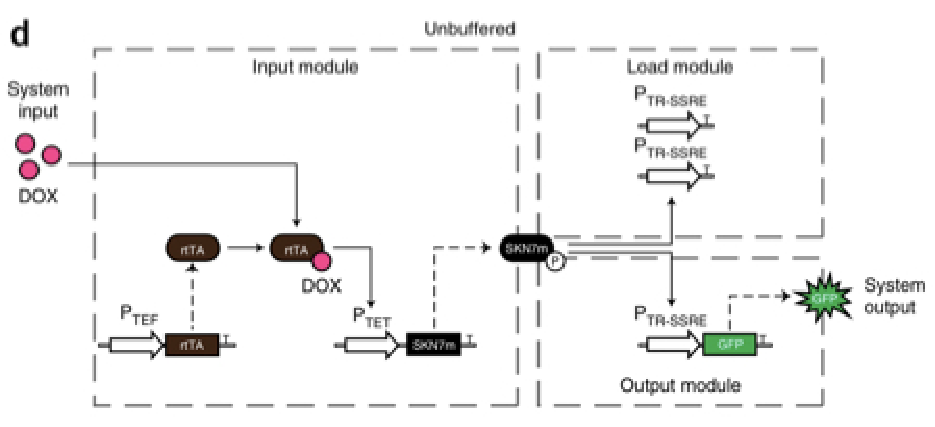
\includegraphics[width=0.6\textwidth]{unbuffered_diagram.pdf}
\end{center}

To put this in more formal terms, suppose the output of the first module is the production rate $x(t)$ for a transcription factor protein $Y$. The concentration of $Y$ would ideally reflect $x(t)$, and assuming that $Y$ undergoes degradation/dilution at a rate $\delta$ and no other reactions, then at steady state, $Y=x/\delta$. However, if $Y$ is capable of binding to a bunch of transcription factor binding sites (which have a total concentration $b_{\textrm{tot}}$ to form a complex $c$, then
\[ \frac{dy}{dt} = x(t) - \delta y { \color{red} + k_{\textrm{off}} c - k_{\textrm{on}} \left( b_{\textrm{tot}} - c \right) y } \]
The last two terms in red represent the feedback from the existing transcription factor binding sites back to $y(t)$. $y(t)$ is effectively buffered: these sites will ``soak up" new $Y$ as it's produced and release it as $Y$ degrades. This not good if $y(t)$ is supposed to reflect $x(t)$ and serve as the input to downstream modules.

\begin{center}
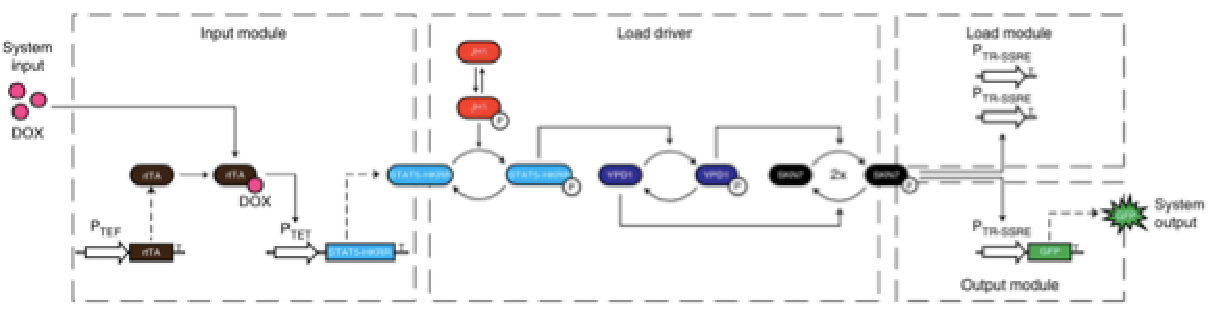
\includegraphics[width=0.8\textwidth]{buffered_diagram.pdf}
\end{center}

Mishra et al. (2014) demonstrate how this issue can be alleviated using an intermediate between the upstream and downstream modules that includes a phosphorylation cycle. To illustrate the mechanism, we follow the chapter by Del Vecchio and Sontag (2010) which will be posted to the course website. Suppose that the output of the upstream module is the production rate $x(t)$ of a kinase $K$. $K$ will undergo first-order degradation so that its steady-state concentration is $K=x/\delta$. $K$ converts an inactive transcription factor $Y$ to its active form $Y^*$, which can bind DNA sites $B$. $Y^*$ can also be acted on by a phosphatase $P$:
\[ \ce{Y + K ->[k_1] Y^{*} + K} \hspace{3 cm} \ce{Y^* + P ->[k_2] Y + P} \]
We assume that both enzymes are in their first-order regime. Then
\begin{eqnarray*}
 \frac{dy^*}{dt} & = & k_1 K y - k_2 P y^* {\color{red} + k_{\textrm{off}} c - k_{\textrm{on}} \left( b_{\textrm{tot}} - c \right) y^* }\\
 & = & k_1 K \left(y_{\textrm{tot}} - y^* - c \right) - k_2 P y^*  { \color{red} + k_{\textrm{off}} c - k_{\textrm{on}} \left( b_{\textrm{tot}} - c \right) y^* }
 \end{eqnarray*}
The terms in red represent the retroactivity. If we assume that $Y_{\textrm{tot}} \gg B_{\textrm{tot}}$, then
\begin{eqnarray*}
 \frac{dy^*}{dt} & \approx & k_1 K y_{\textrm{tot}}  - k_2 P y^*  { \color{red} + k_{\textrm{off}} c - k_{\textrm{on}} \left( b_{\textrm{tot}} - c \right) y^* }
 \end{eqnarray*}
 Now we introduce the quantities $G=k_1 y_{\textrm{tot}}$ and $G'=k_2 P$. If both are large relative to the other quantities, then:
\begin{eqnarray*}
 \frac{dy^*}{dt} & = & G K  -  y^* G' { \color{red} + k_{\textrm{off}} c - k_{\textrm{on}} \left( b_{\textrm{tot}} - c \right) y^* }\\
 & \approx &G K  -  y^* G'
 \end{eqnarray*} 
and so $y^*$ should accurately reflect $K$, which in turn accurately reflects the output of the upstream module! This basic approach, with some added bells and whistles, was successfully implemented and used to improve performance in a synthetic system in yeast (Mishra et al., 2014).

\begin{center}
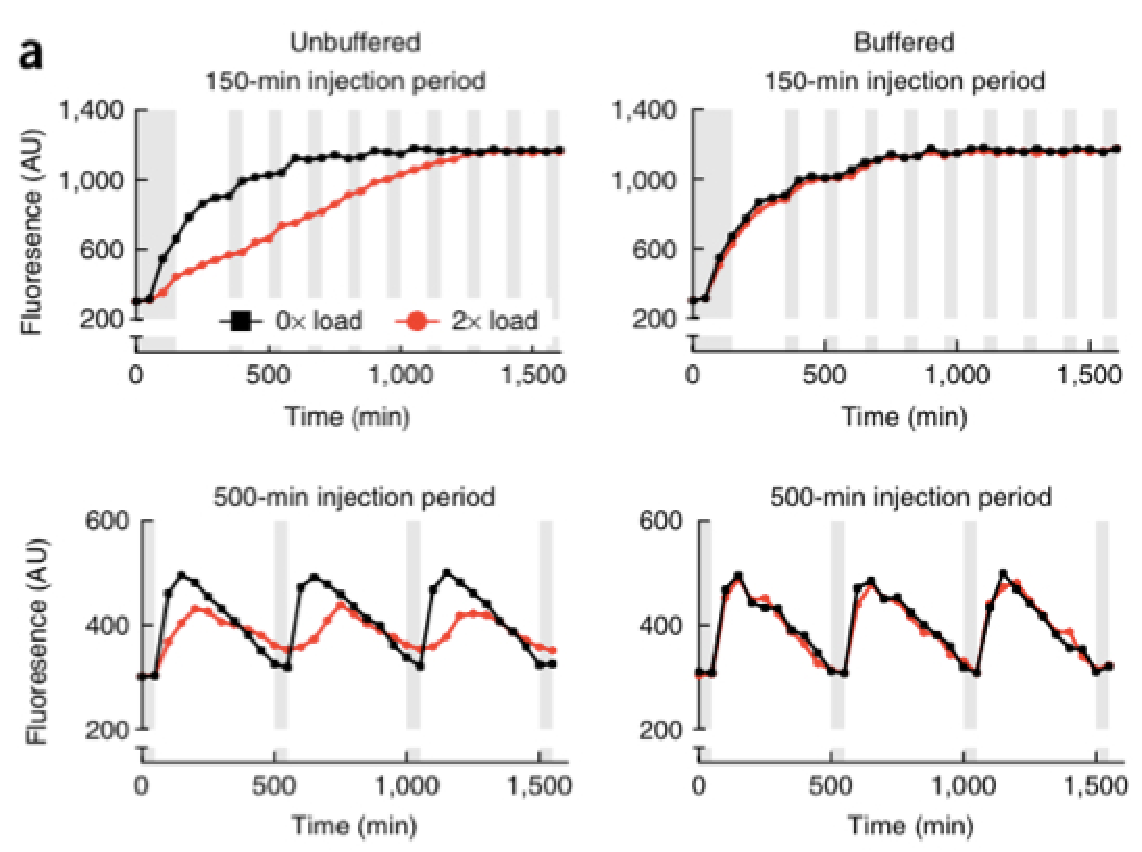
\includegraphics[width=0.7\textwidth]{retroactivity.pdf}
\end{center}

\end{document}